\documentclass[a4paper,12pt]{article}
\usepackage[utf8]{inputenc}

\usepackage[top=2cm,bottom=2cm,right=2cm,left=2cm]{geometry}
\usepackage{amsmath,amssymb,enumitem,multicol,graphicx,tikz,framed,tcolorbox,mathtools,comment,subcaption,array,pgfplots}
\usepackage{listings}
\usepackage{xcolor}
\linespread{1.3}
\setlength\parindent{0pt}
%New colors defined below
\definecolor{codegreen}{rgb}{0,0.6,0}
\definecolor{codegray}{rgb}{0.5,0.5,0.5}
\definecolor{codepurple}{rgb}{0.58,0,0.82}
\definecolor{backcolour}{rgb}{0.95,0.95,0.92}

%Code listing style named "mystyle"
\lstdefinestyle{mystyle}{
  backgroundcolor=\color{backcolour},   commentstyle=\color{codegreen},
  keywordstyle=\color{magenta},
  numberstyle=\tiny\color{codegray},
  stringstyle=\color{codepurple},
  basicstyle=\ttfamily\footnotesize,
  breakatwhitespace=false,         
  breaklines=true,                 
  captionpos=b,                    
  keepspaces=true,                 
  numbers=left,                    
  numbersep=5pt,                  
  showspaces=false,                
  showstringspaces=false,
  showtabs=false,                  
  tabsize=2
}

%"mystyle" code listing set
\lstset{style=mystyle}


\usepackage{lipsum,hyperref}
\hypersetup{
	colorlinks=true,
	linkcolor=blue,
	filecolor=magenta,      
	urlcolor=cyan,
}

\begin{document}
	\Large \textbf{Advanced Processes:}\normalsize\\\\
Looking at the Merit criteria for this standard:
\begin{itemize}
	\item 	effectively using project management and version control tools and techniques to manage the development of a digital technologies outcome
	\item trialling multiple components and/or techniques and selecting those which are
	most suitable
	\item using information appropriately from testing and trialling to improve the
	functionality of the digital technologies outcome
	\item addressing relevant implications.
\end{itemize}
The project management technique we will use will be the Agile technique.\\
Our version control is Git hub (watch videos and make the repository in the video)\\
Relevant implications will be similar to last year\\

\section{Agile}
Much of this material has come from Atlassian \url{https://www.atlassian.com/agile}\\\\
Agile is fundamentally team based, but you can apply its thinking and methods to your individual projects.\\\\
Agile originally came from a ``manifesto'' of software developers in 2001. \\
At that stage software development involved:
\begin{itemize}
	\item complete planning of the project before starting to make anything, 
	\item long deadlines (six months or more), 
	\item generally only seeing the clien at the beginning and at the end of a project,
	\item  members of the team had highly specified rolls (`` I only do databases'').
\end{itemize}
The problem with this (Waterfall) approach is that building digital products is still a new area
\begin{itemize}
	\item  So that new needs or technical approaches can emerge at any time and people often learn as they go.
	\item By the time the client gets the product, it is out of date and is inflexible to new requirements or changes.
	\item The product is not being tested in the marketpalce until it is finished
	\item During the project, some team members will have lots to do whilst others are doing little because the needs are outside of their job description
\end{itemize}
Some of the fundemental ideas behind agile are
\begin{itemize}
	\item A team is a \textbf{TEAM}. So members should be aware of what others are doing, may fast track actions so that another part of the team is not \textbf{blocked} and may take on different non-specialist rolls at different times.
	\item The emphasis is on working software (applications) that can be launched quickly and developed upon responsively to the market place and clients needs (have you ever had to download an update??)
	\item Being responsive to change (have a plan but change the plan if it is the right thing to do)
\end{itemize}
This is the general idea of Agile and its actual implementation is done using methodologies such as \textbf{Scrum} and \textbf{Kanban}.\\
We will use Scrum.
\subsection{Scrum}
All agile methods follow similar patterns.
\begin{itemize}
	\item Break the project down into small parts (project backlog)
	\item Prioritize
	\item Plan and implement a short passage of work that will have a tangible outcome (sprint)
	\item Have regular, quick meetings or reviews ``standups'' to identify 
	\begin{itemize}
		\item What have I done (yesterday)?
		\item What do I intend to do next (today)?
		\item What is blocking me?
	\end{itemize}
	\item Review completed passage of work (sprint review)
	\item Repeat the cycle (iterate)
\end{itemize}

\newpage
\section{Let's consider a brief}
	
Amy has an  large bowl of fruit at home.\\
It currently contains 5 Apples , 7 Pears , 2 Mangoes, 9 KiwiFruit and 3 Peaches.\\
Amy would like a program designed so that she monitor the consumption of her fruit.\\\\

We are assuming that we will make this in Python and that it will be a console program.\\
However, we can think a little more widely before we start.\\
Using a brainstorming process we can think about all the things we would like the program to do.\\
We then break these ideas up into pieces and place them in a \textbf{Project Backlog}
	\subsection{Project Backlog}
	\begin{itemize}
		\item The project backlog is a list of all the things the program might do.
		\item It can (theoretically) be infinite in size
		\item The project backlog can be updated regularly during a project
		\item The project backlog should also contain the \textbf{simplest possible} ideas for the project
		\item The project backlog should be ordered by \textbf{priorities}, most essential at the top, working down
	\end{itemize}
\begin{figure}[!ht]
	\centering
	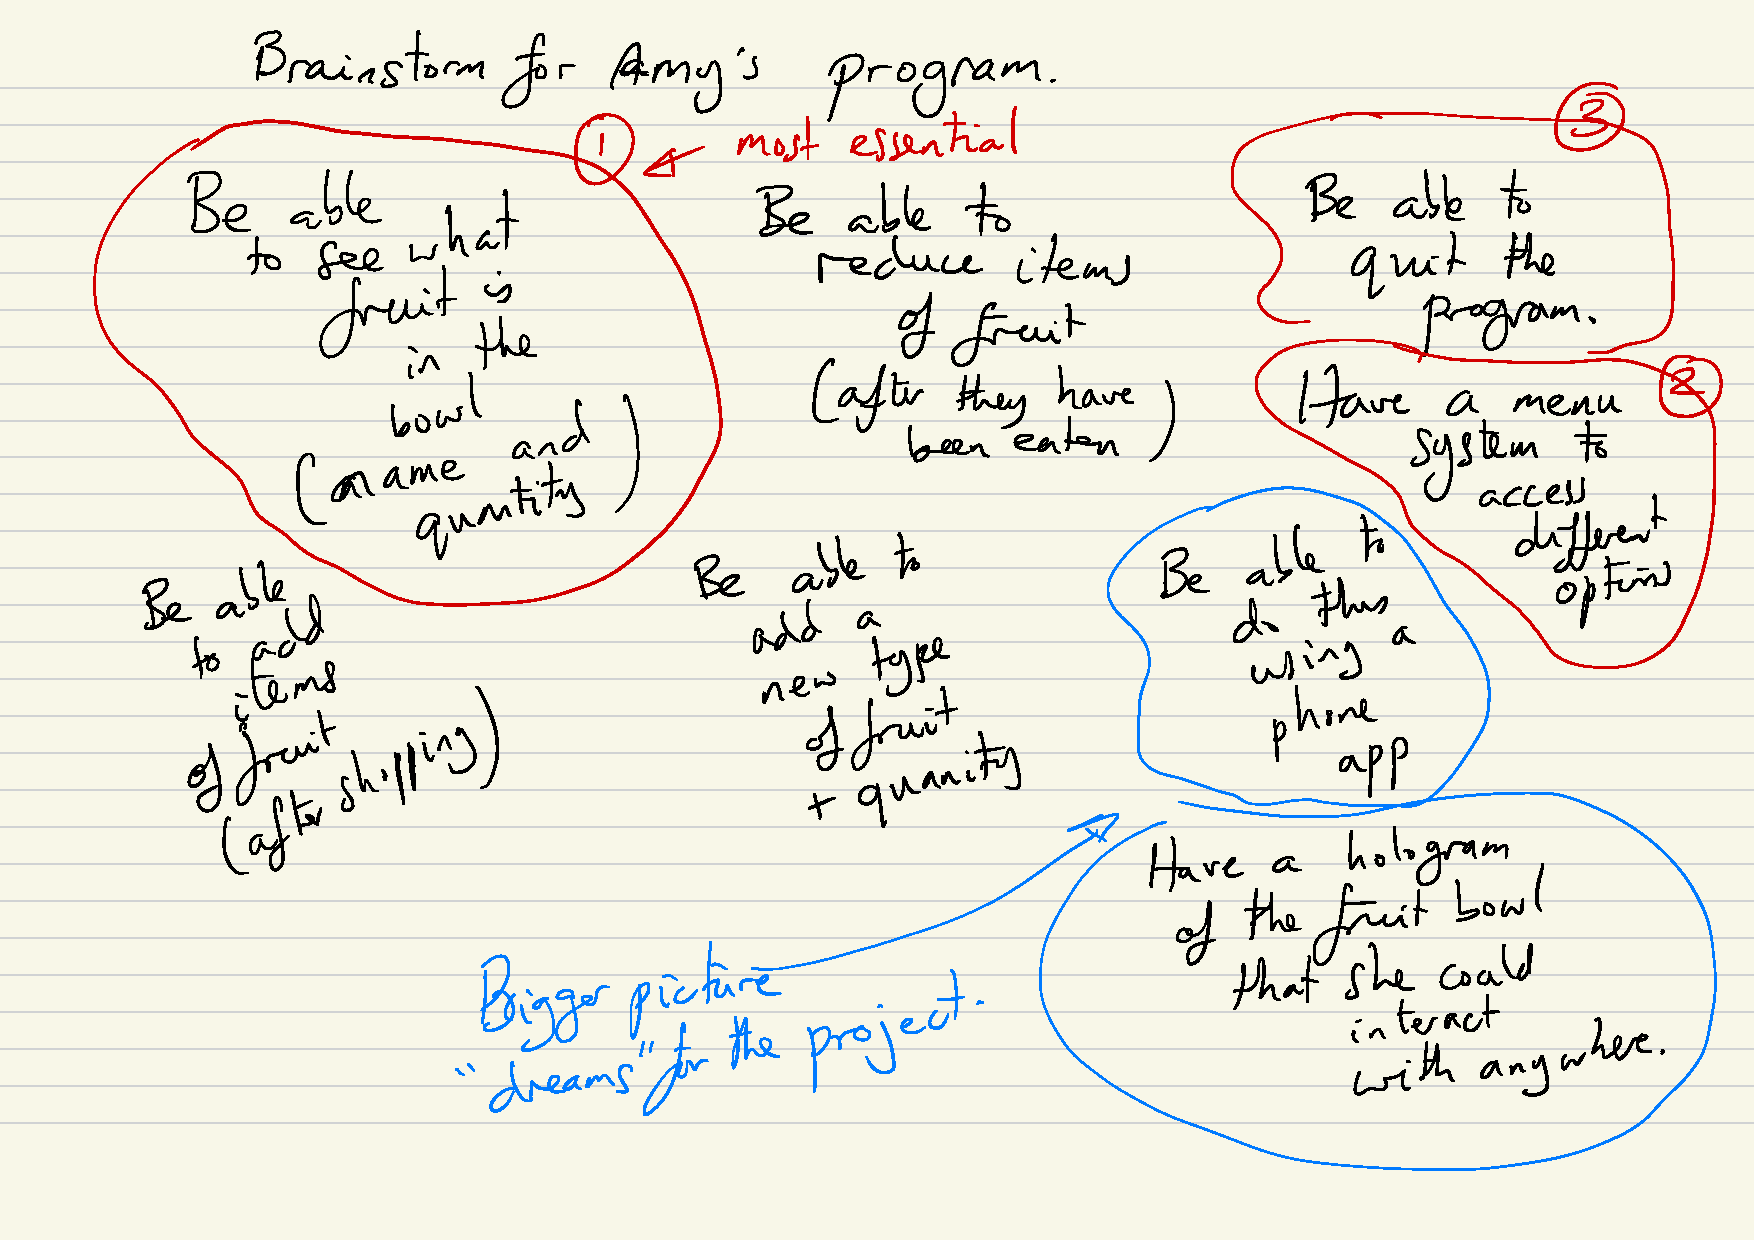
\includegraphics[width=11cm]{brainstorm_plan.pdf}
\end{figure}

The project backlog gets set up as a trello/kanban whetever type board.
\begin{figure}[!ht]
	\centering
	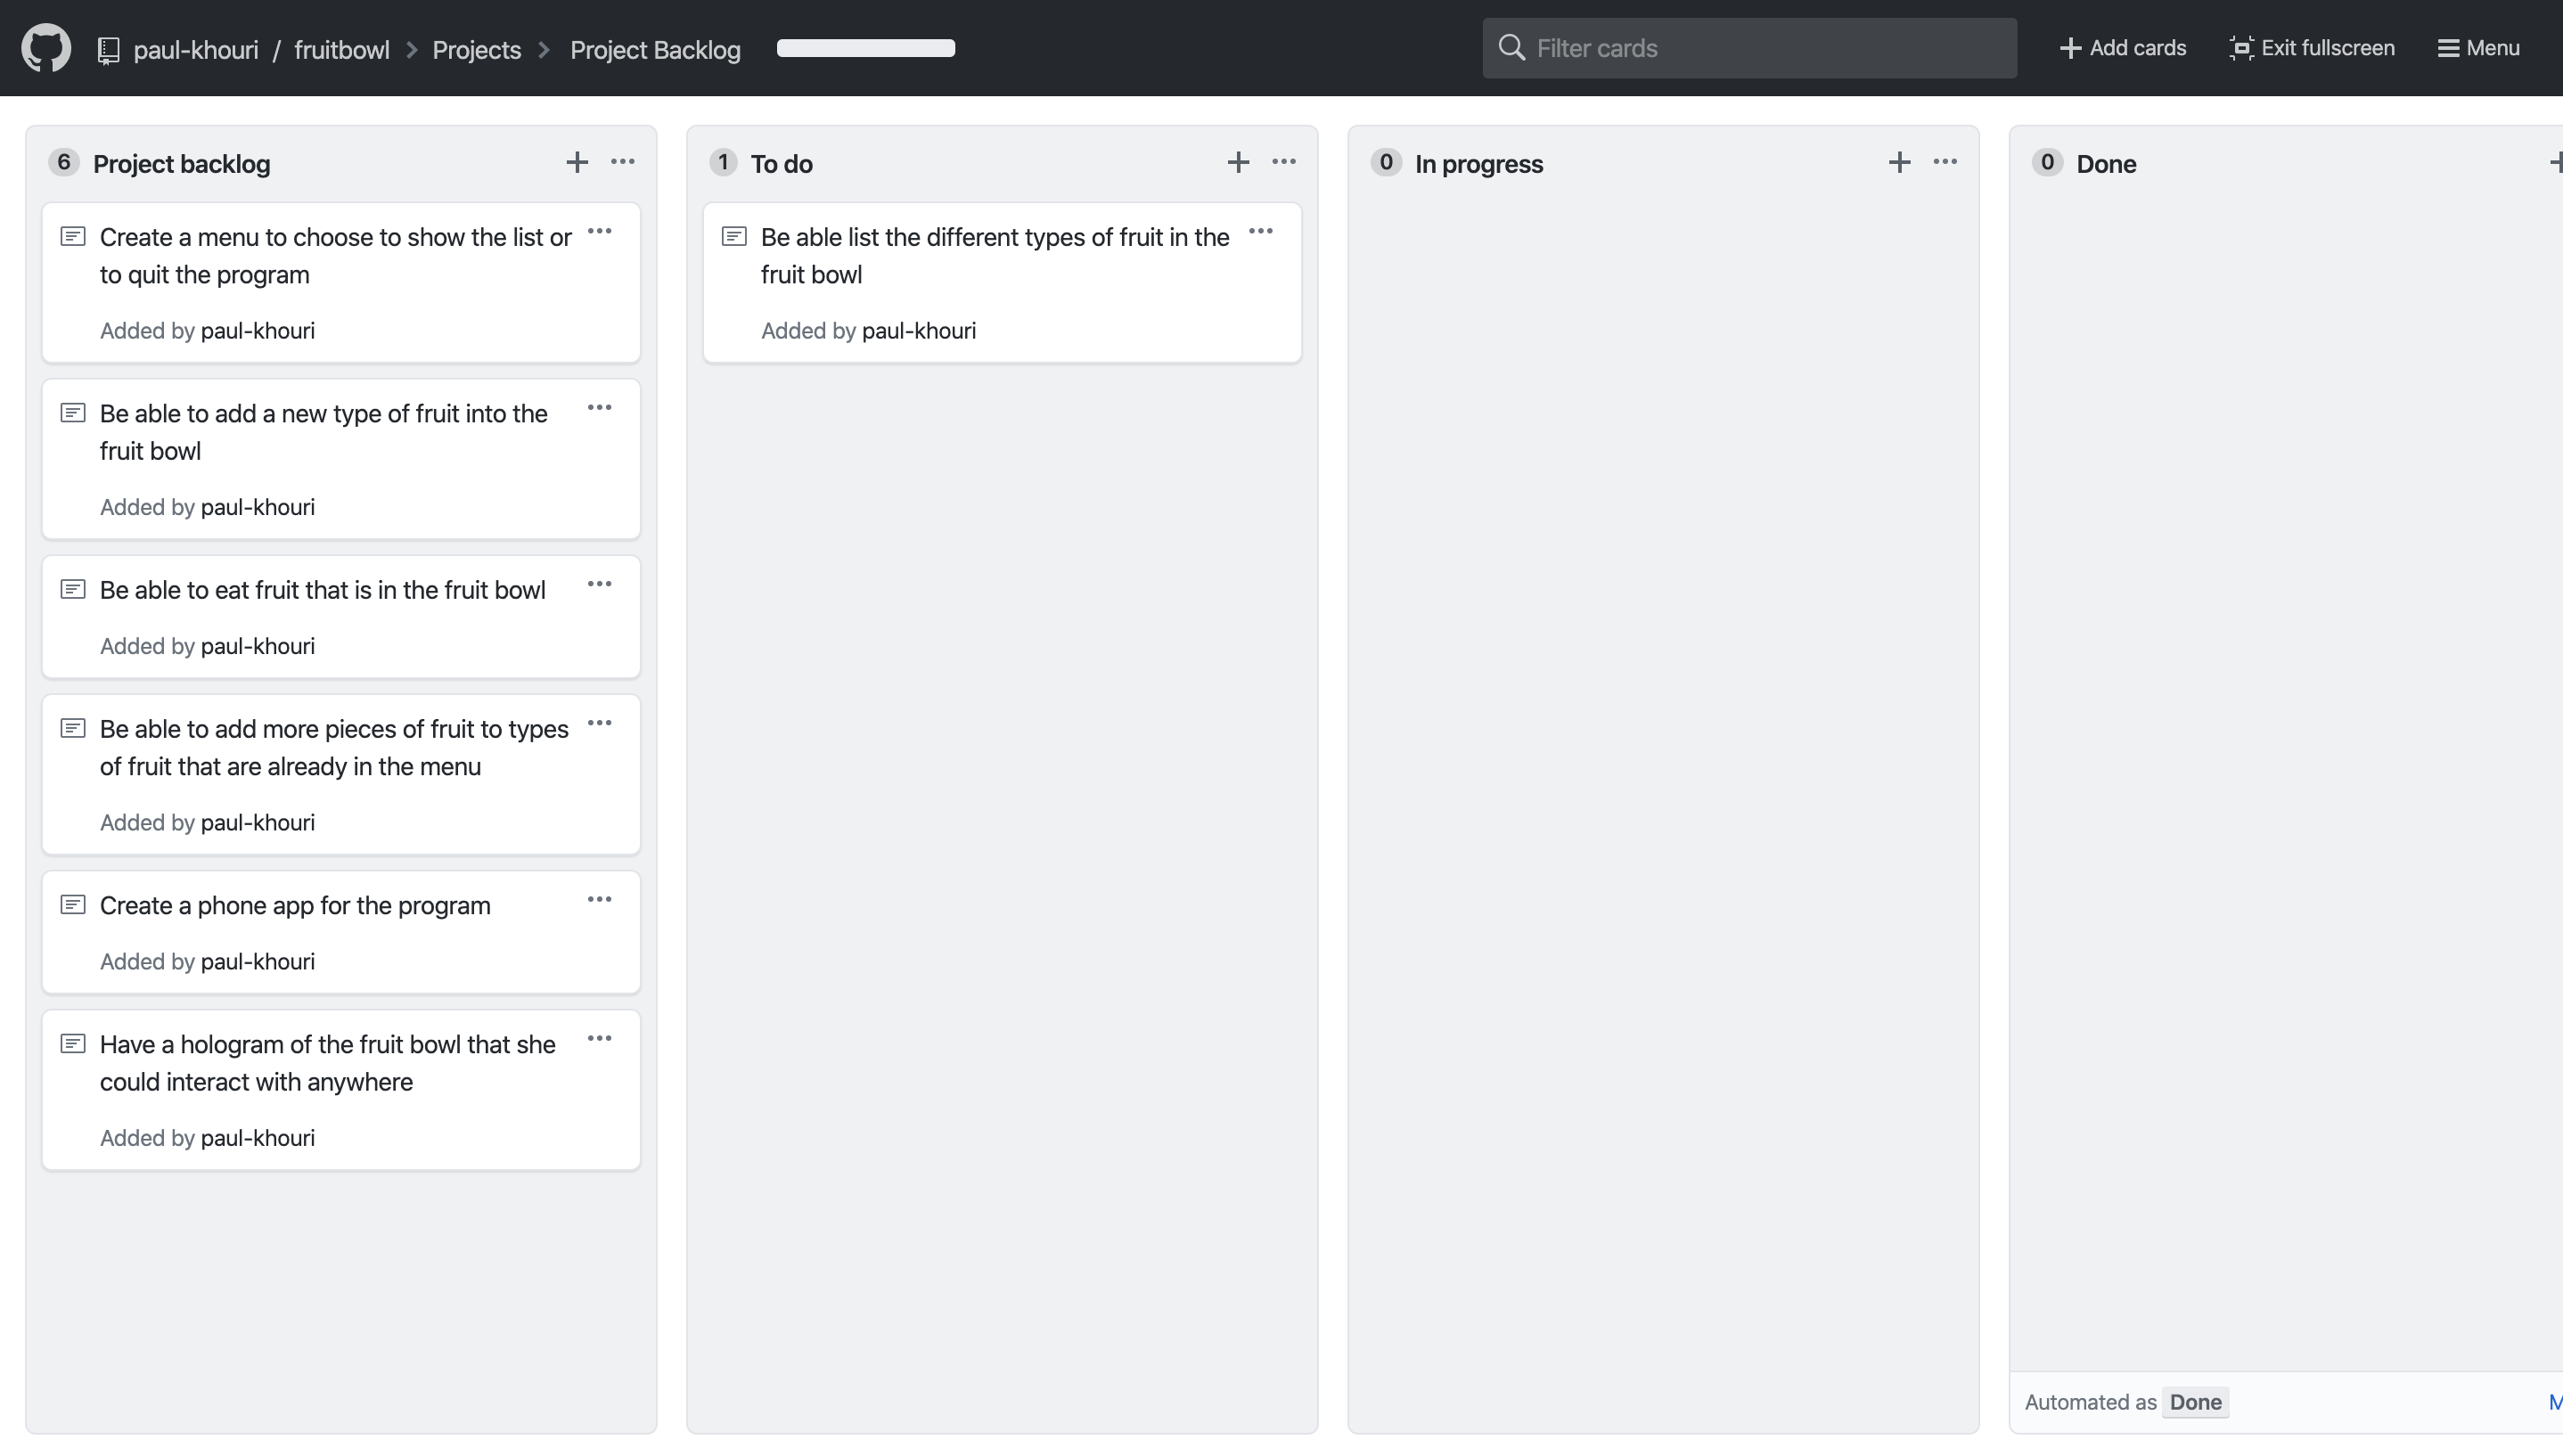
\includegraphics[width=11cm]{Project_backlog.png}
\end{figure}
	
\subsection{The Sprint}
\begin{itemize}
	\item A sprint is a planned passage of work that is completed in a short timeframe and leads to a tangible outcome.
	\item It ``adds value'' to the project.
	\item Ideally we should take the highest priority item in the project backlog (as our sprint) and plan to complete it in a short period of time (2 or 3 days).
	\item Ideally the project backlog is being updated to break things down into achievable pieces.
\end{itemize}
\subsection{Sprint 1}
Taking the aim ``to list the contents of the fruit bowl'' , we plan the sprint , then do it.\\
Every sprint should follow the requirments below\\
Not every sprint needs to be documented in meticulous detail, but \textbf{key} sprints should be.\\\\
You want to include:
\begin{itemize}
	\item Aim
	\item Trello or Kanban Board
	\item  Natural language sketch planning
	\item Standup comments
	\item  Testing
	\item Sprint Review
\end{itemize}
\begin{figure}[!ht]
	\centering
	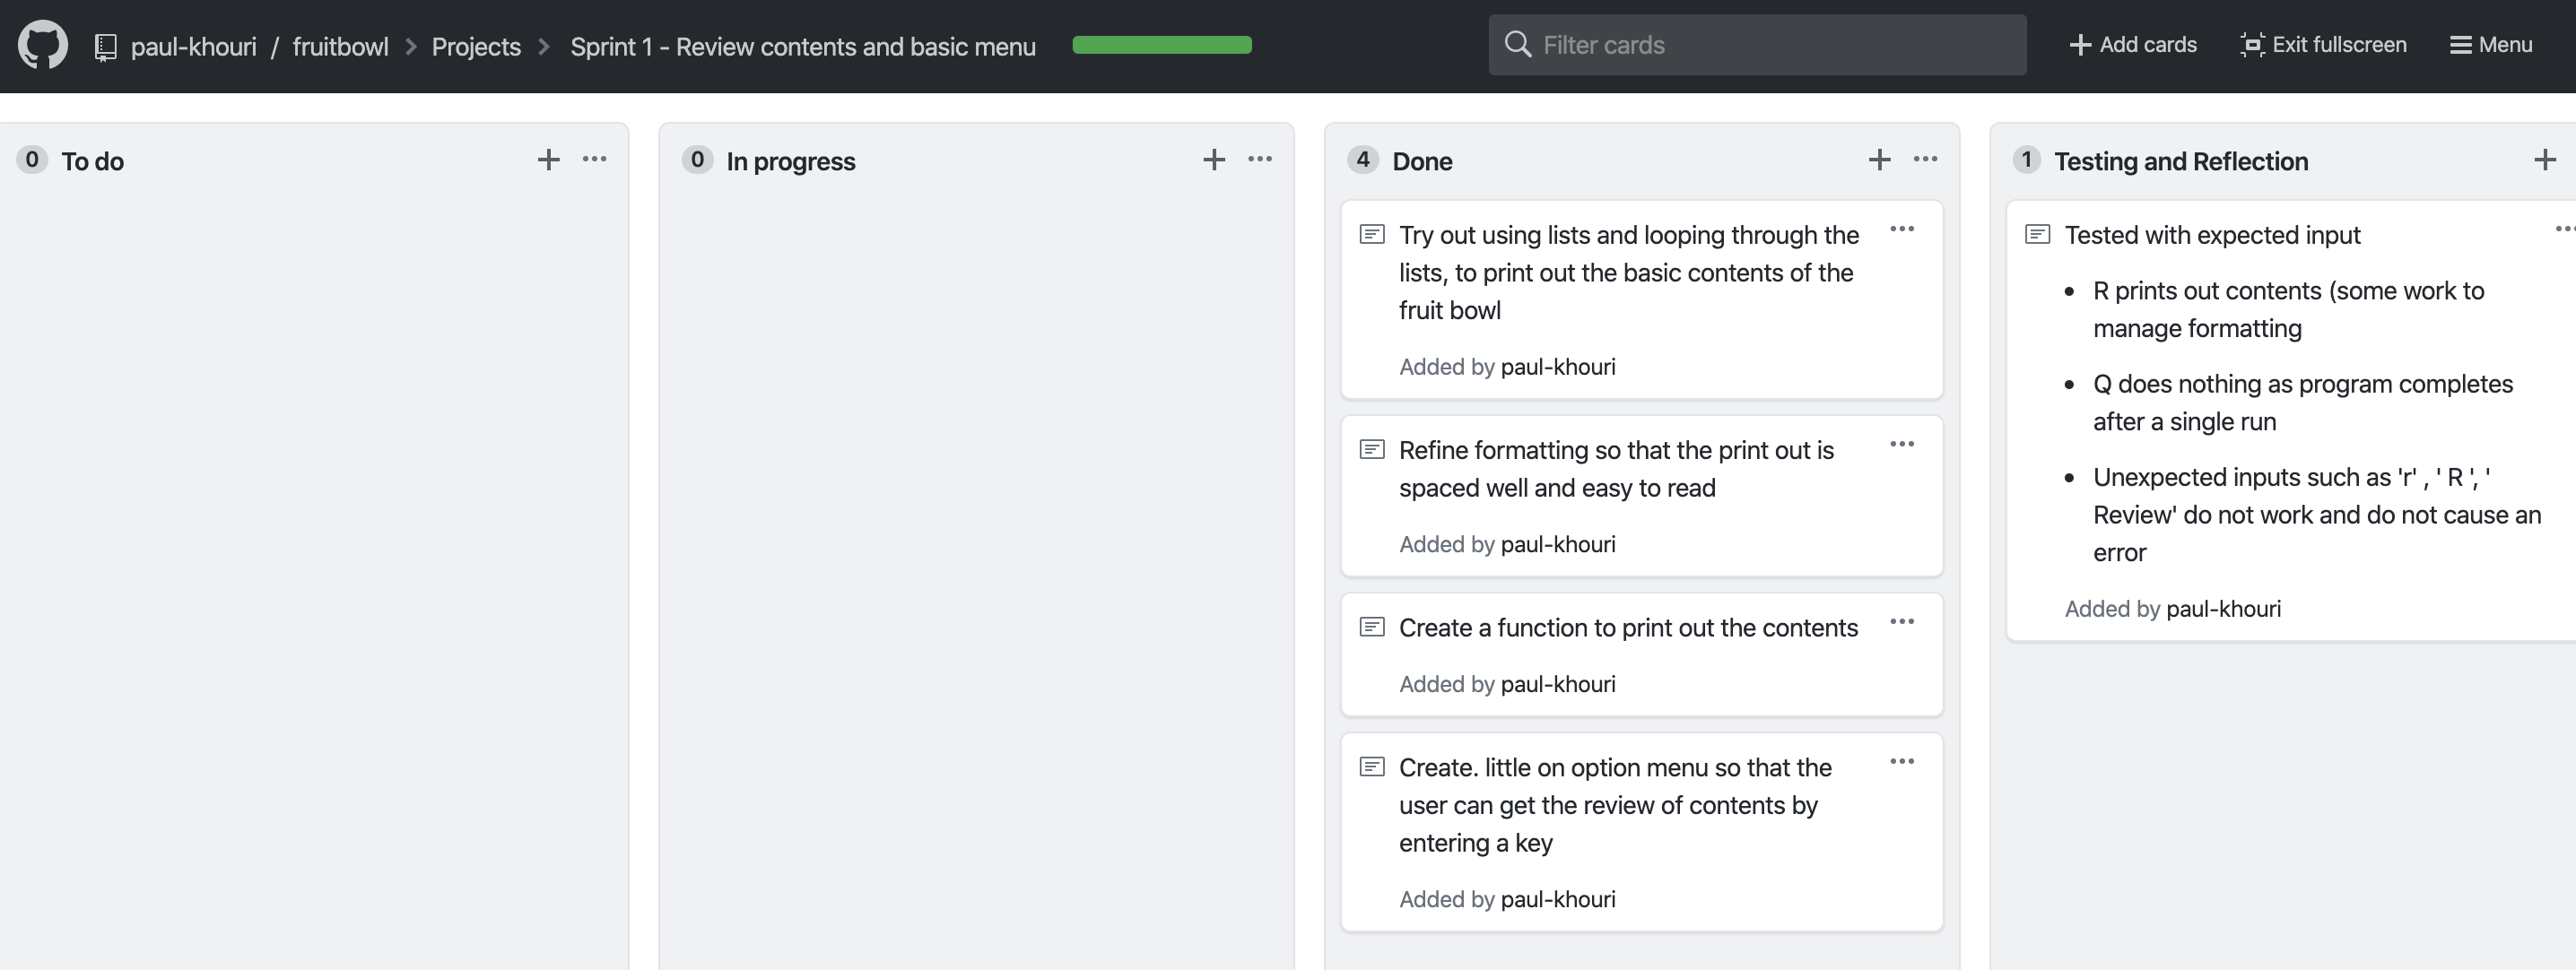
\includegraphics[width=16cm]{images/board_1.png}
\end{figure}
\begin{figure}[!ht]
	\centering
	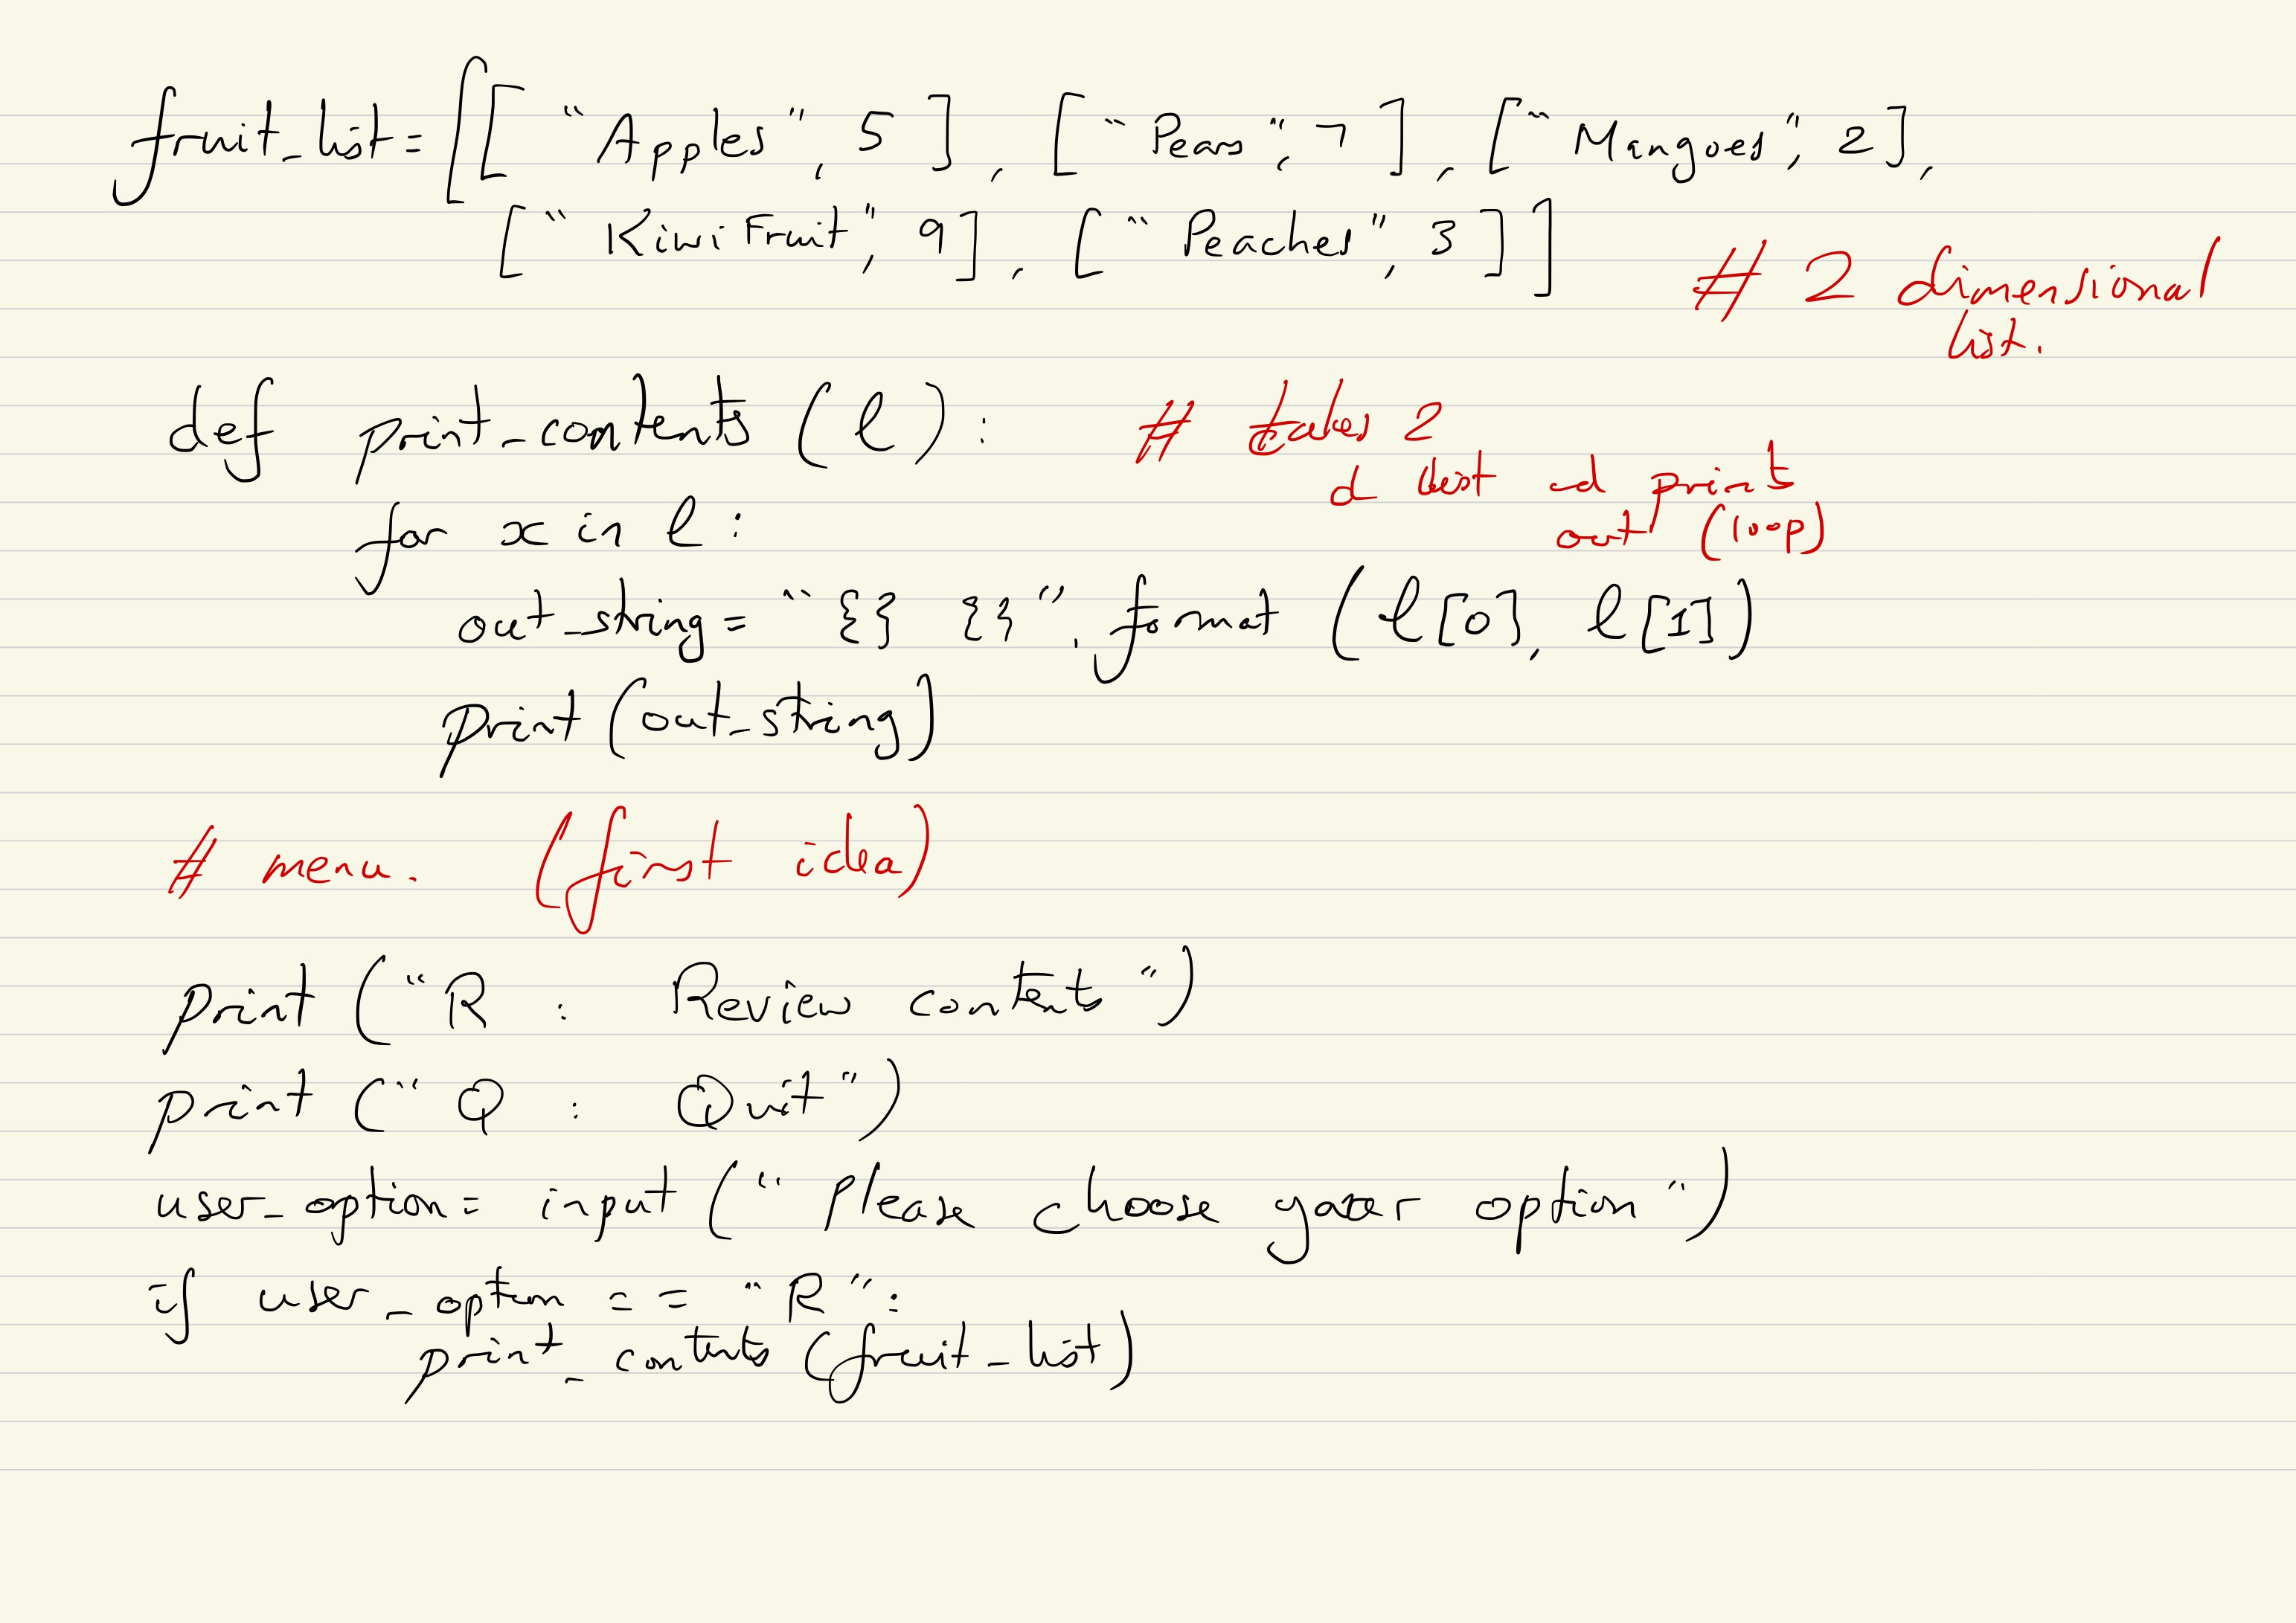
\includegraphics[width=14cm]{images/Sprint_1_plan.jpg}
\end{figure}
\newpage
\lstinputlisting[caption = Successful Test]{images/sprint_1_test.txt}
\subsection{After the sprint (sprint review)}
\begin{itemize}
	\item The project backlog should be reviewed and updated.
	\item The top of the backlog is taken for the next sprint.
	\item Files are uploaded to github and commits periodically documented
\end{itemize}

\section{Running the project overall}
We follow a cycle of sprint after sprint, building up the sophistication of the program.\\
In the case of our fruit bowl the sprints would be somthings like:
\begin{itemize}
	\item Allow the user to add an amount of a fruit  (i.e choose a fruit and add a certain amount)
	\item Allow the user to remove an amount of a fruit  (i.e choose a fruit and remove a certain amount)
	\item Allow the user to add a new type of fruit
	\item Allow the user to remove a type of fruit.
	\item At some stage improve the menu structures.
	\item At some stage review the structure of the program and re organise if necessary
	\item Manage user interaction so that inputs are validated and assist the user 
\end{itemize}

\begin{figure}[!ht]
	\centering
	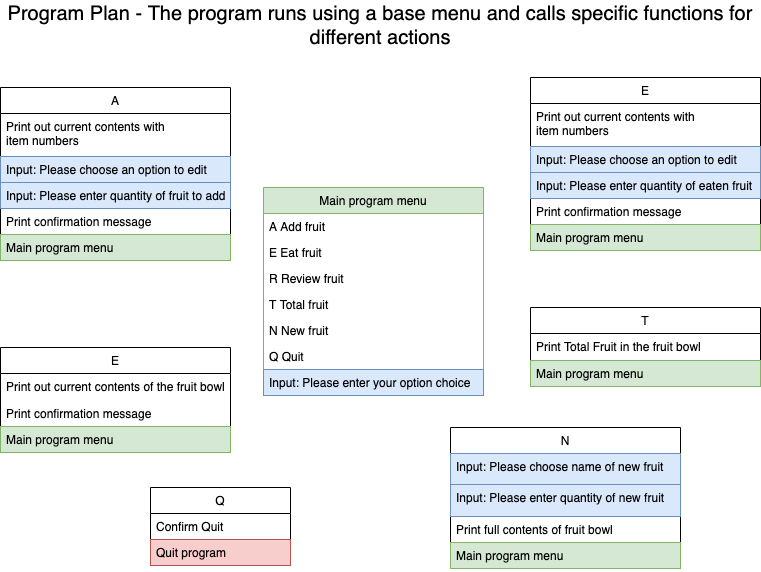
\includegraphics[width=12cm]{images/GeneralPlanning-Fruit_Structure.png}
\end{figure}
Each sprint could, in theory, been seen as the process of creating one of these functions.\\
Validation functions would also have to be built.
\newpage
\subsection{A sprint for adding fruit to the fruit bowl}
Aim: For the user to be able to add fruit to the fruit bowl. The component should print out the current contents of the bowl, allow the user to choose which fruit they want to add to, add some fruit and then get confirmation.\\
Once the function is working properly, move it into the main version and connect it with the main menu through a function call. 

\lstinputlisting[caption = Code outline for add fruit function]{images/adding_fruit_pseudo.txt}
\begin{figure}[!ht]
	\centering
	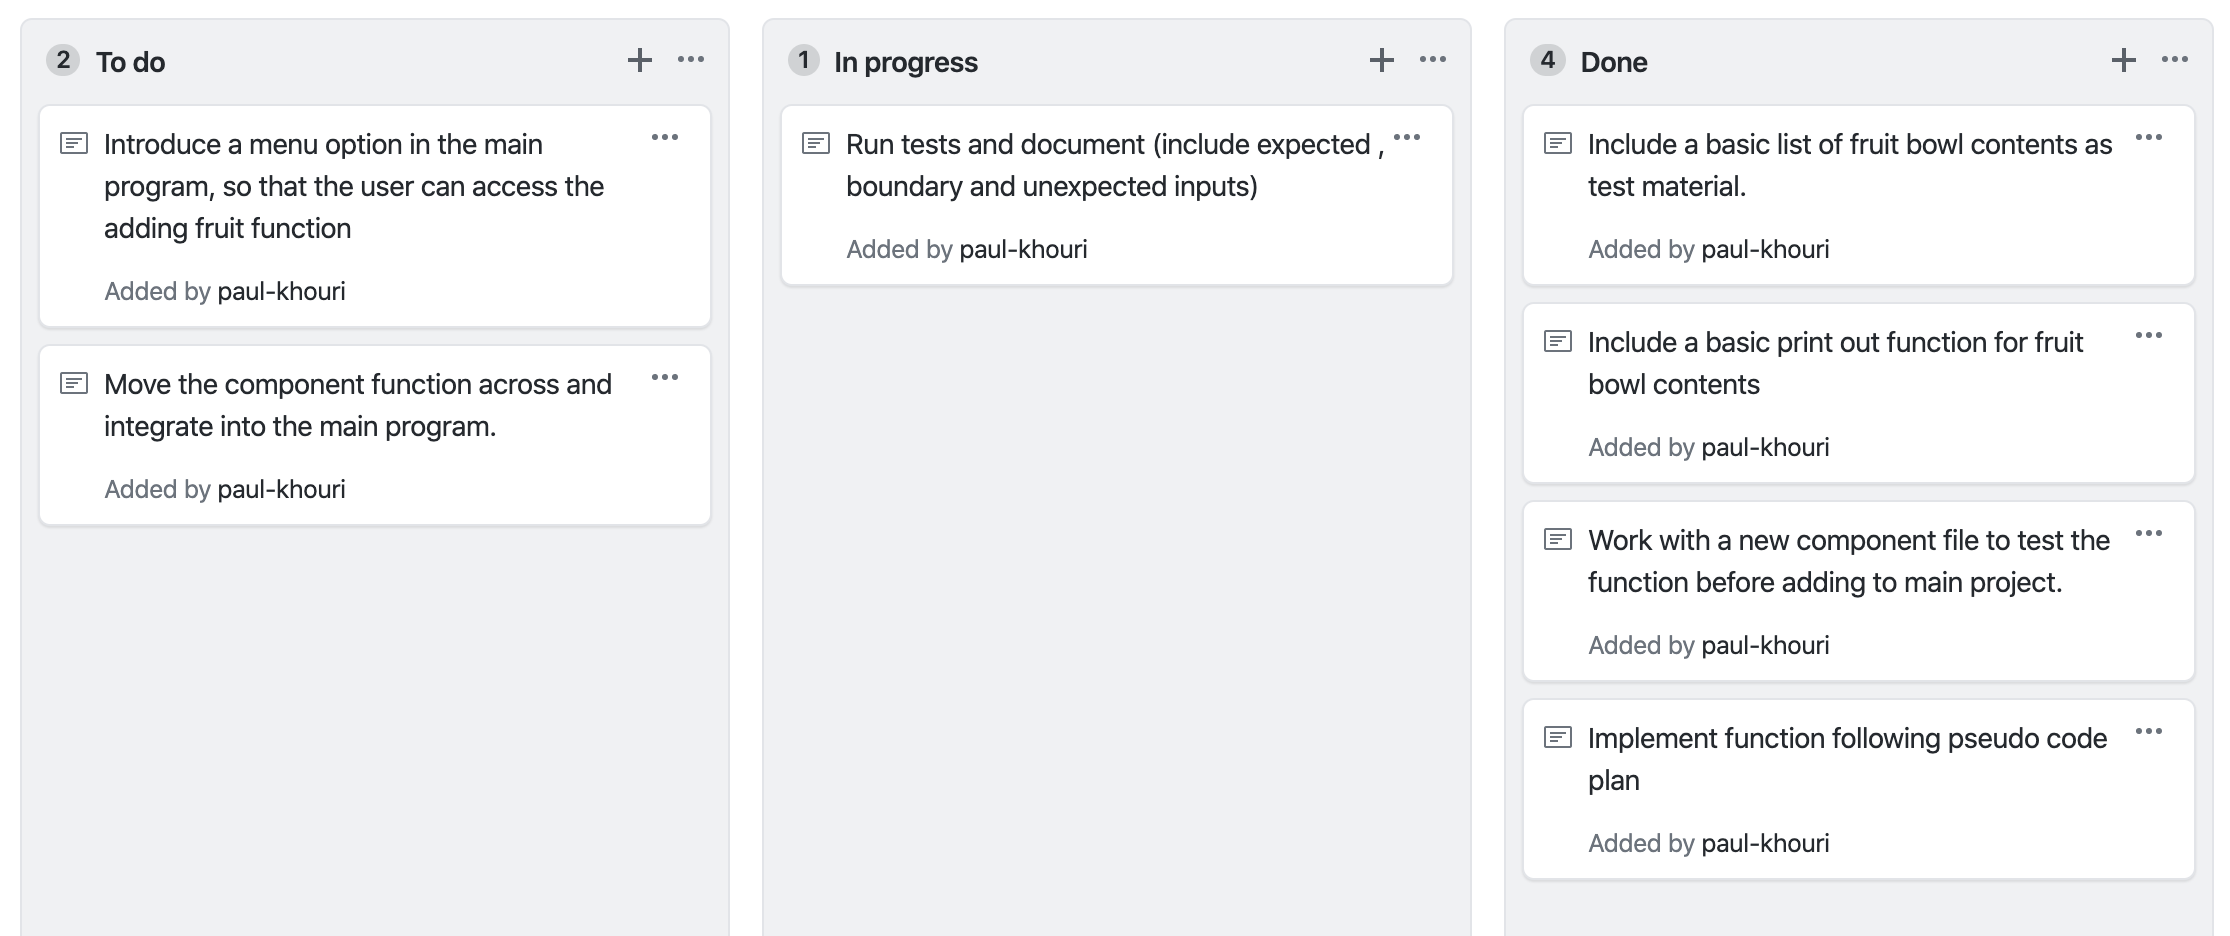
\includegraphics[width=14cm]{images/Adding_fruit_board.png}
\end{figure}
\subsubsection{Testing}
Basic principles of testing:
\begin{itemize}
	\item Testing exists to find errors in a program (not to avoid finding errors).
	\item Tests should consciously seek to find errors by exploring different input patterns.
	\item We have a general principle of testing for \textbf{expected} , \textbf{boundary} and \textbf{unexpected} inputs
	\item Complete the tests you have planned before trying to fix errors.
	\item Not all tests need to be documented in detail, but you must demonstrate solid evidence of good testing processes in your overall planning work.
\end{itemize}
\newpage

\begin{figure}[!ht]
	\centering
	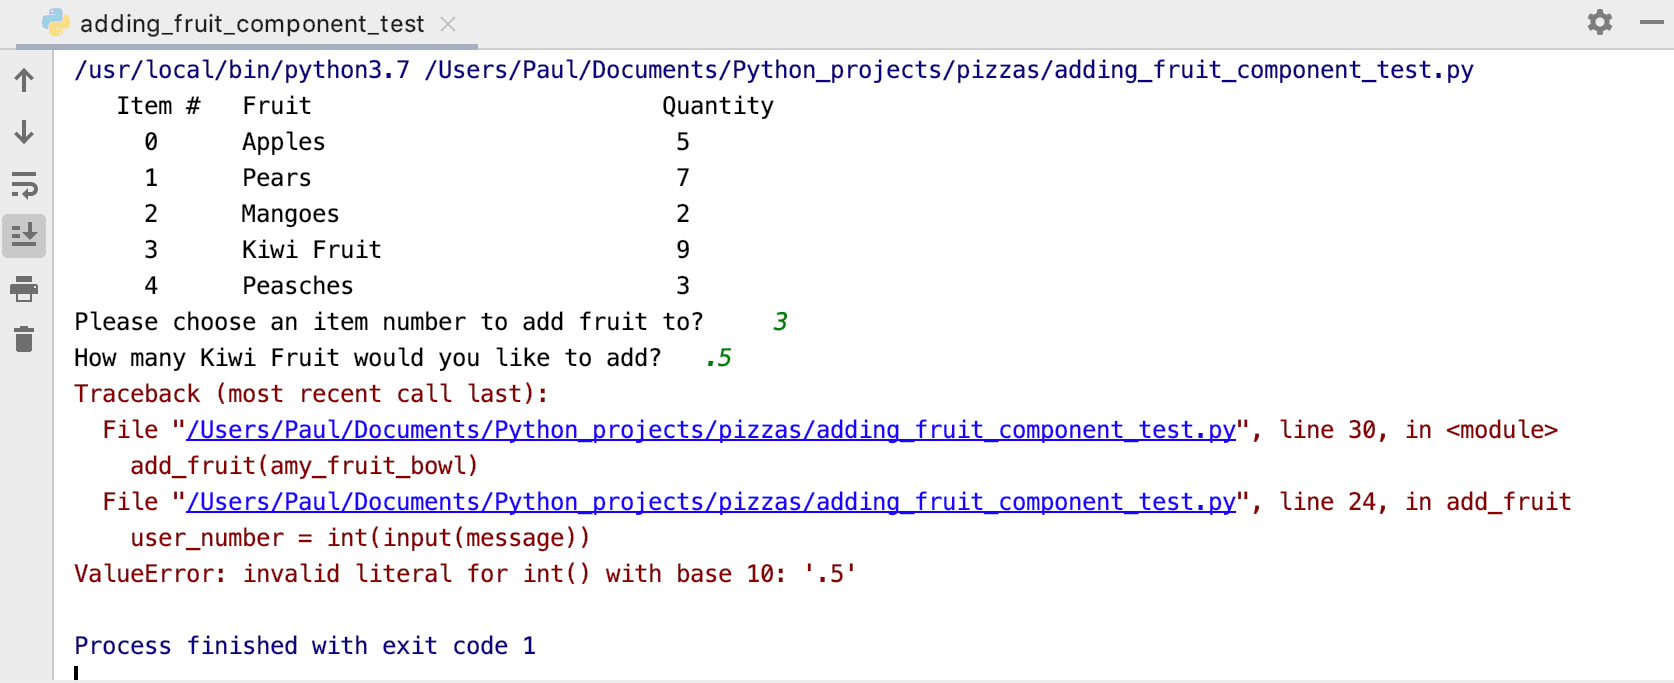
\includegraphics[width=14cm]{images/adding_fruit_test_1.png}
\end{figure}
Test looking at entering .5 rather than 5 for adding to the Kiwi Fruit. The integer cast leads to a program crash. This needs fixing.\\

\begin{figure}[!ht]
	\centering
	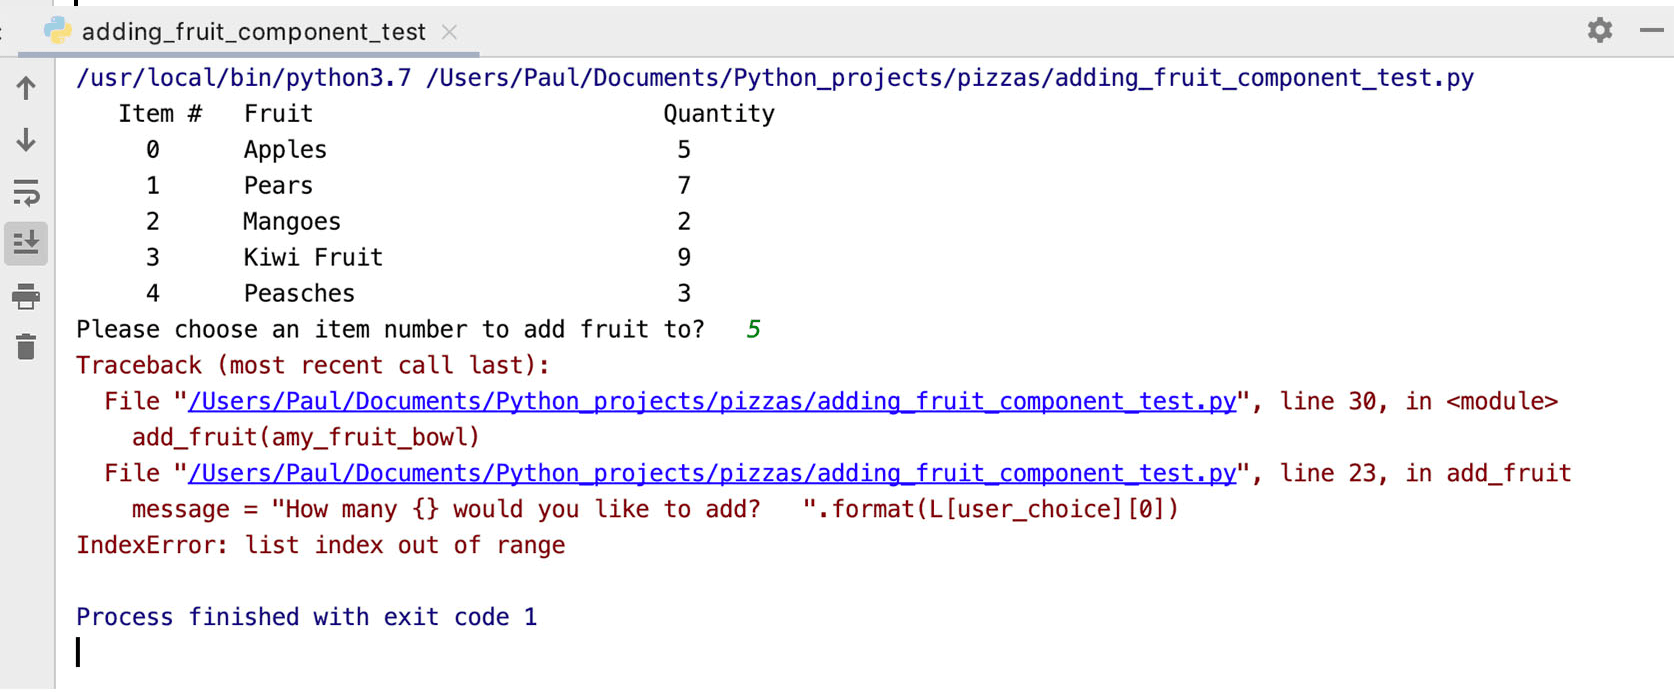
\includegraphics[width=14cm]{images/adding_fruit_test_2.png}
\end{figure}
Looking at entering an item value that is not is on the menu list. This is calling an index that doesn't exit on the fruit bowl list. This leads to a ``index out of range'' crash.\\

\begin{figure}[!ht]
	\centering
	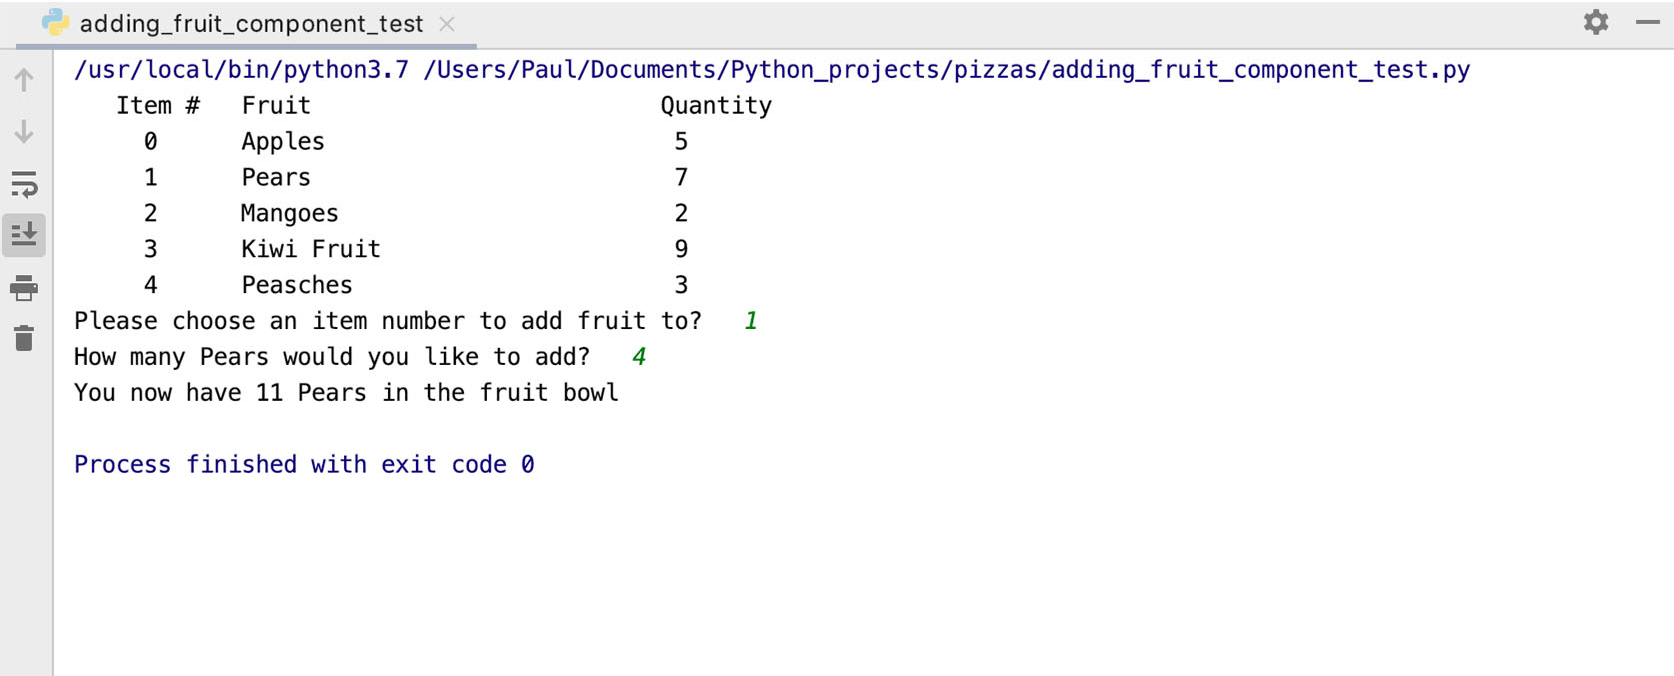
\includegraphics[width=14cm]{images/adding_fruit_test_3.png}
\end{figure}
Expected input test, works correctly.\\

\subsubsection{Sprint Review}
The problems with program crashes with unexpected input and starting to annoying. \\
Solution: move validation (which helps the user by prventing errors, or giving feedback on how to detect errors) up the project backlog and make this the nest sprint.
\section{Component Testing}
\section{Version Control}
Git is a mangement environment that tracks the history of file versions 






	
	
	
	
	
	
	
	
	
	
	
\end{document}